\chapter{Direct transfer analysis}

This chapter presents the direct transfer analysis performed on the two
discovered interstellar objects, 1I/'Oumuamua and 2I/Borisov. The algorithm used
is the one devised by \cite{izzo2015}, as it is proven to be more accurate and
faster than other classical algorithms \cite{martinez2021}. The ephemerides for
1I/'Omuaumua and 2I/Borisov are obtained from JPL Horizons API service. These
are propagated under the two-body assumption to simplify the analysis.
Propagation starts on January 1, 2016 and ends on January 1, 2035.

The analysis includes porkchop plots for quickly visualizing different mission
constraints. The optimum transfers are computed and their figures are generated
for better undesrtanding the orbit. A short discussion on the obtained values is
presented at the end of the chapter.

\section{Characteristic energy at launch}

The characteristic energy for launch is the energy required to set a spacecraft
into the desired targeting orbit. This analysis assumes that the spacecraft
launches from Earth, which is modeled as a point with no mass and arrives at the
target interloper, modeled again as a massless point. The only force acting on
the spacecraft is the gravitational force of the Sun.

Before launching, the spacecraft has the velocity of Earth, $\vec{v_{\oplus}}$.
At launch, the spacecraft presents an heliocentric velocity $\vec{v_{\infty
,1}}$ that matches the solution of Lambert's problem. Vector $\Delta{\vec{v}}$
is the difference between the two velocities, and its modulus matches the
required impulse velocity, as stated in Equation \ref{eq:launch_velocity}.

\begin{equation}
    \Delta v_1 = \|\vec{v_{\infty ,1}} - \vec{v_{\oplus}}\|
    \label{eq:launch_velocity}
\end{equation}

The value of $\Delta v_1$ can be used in Equation \ref{eq:c3} for solving the
characteristic for launch.

\subsection{'Oumuamua}

Porkchop plots for 1I/'Oumuamua representing the characteristic energy for launch
are shown in figure \ref{fig:oumuamua-direct-prograde-transfer-porkchop} and
figure \ref{fig:oumuamua-direct-retrograde-transfer-porkchop}.

\begin{figure}[H]
  \centering
  \includegraphics[width=\textwidth]{static/oumuamua/direct-prograde-transfer-porkchop.png}
        \caption[Direct and prograde launch energy porkchop for 'Oumuamua]{Launch energy porkchop plot for 1I/'Oumuamua for a direct and prograde
        transfer showing the isolines for
        the time of flight required for a targeting. A region of low transfer
        energy is located in the lower left corner.}
  \label{fig:oumuamua-direct-prograde-transfer-porkchop}
\end{figure}

\begin{figure}[H]
  \centering
  \includegraphics[width=\textwidth]{static/oumuamua/direct-retrograde-transfer-porkchop.png}
        \caption[Direct and retrograde launch energy porkchop for
        'Oumuamua]{Launch energy porkchop plot for 1I/'Oumuamua for a direct and
        retrograde transfer showing the isolines for
        the time of flight required for a targeting.}
  \label{fig:oumuamua-direct-retrograde-transfer-porkchop}
\end{figure}

In figures \ref{fig:oumuamua-direct-prograde-transfer-porkchop} and
\ref{fig:oumuamua-direct-retrograde-transfer-porkchop}, shorter time of flights
require higher characteristic energies for launch. One may think that a
retrograde transfer orbit would be more efficient considering that 'Oumuamua has
this kind of inclination. However, retrograde orbits do not benefit from Earth's
velocity at launch, which makes them less efficient. Therefore, characteristic
energies for retrograde transfers are higher than for prograde transfers.

Both porkchop plots present a pattern whose solutions alternate between low and
high characteristic energies. This pattern is a consequence of the relative
position of the earth with respect to the target. Low energy solutions
correspong to positions in which the velocity of the Earth gets aligned with the
launch velocity vector.

Note that, despite some areas in the figures not being colored, they have a
solution. These areas do not show any color due to the upper limit for the characteristic
energy at launch imposed of $C_3 = 10000$ km$^2$/s$^2$, imposed by the
author. This allows for a better representation of the porkchops to visually
identify regions. This allows to identify a small region, between years 2016 and
2018 where values for $C_3$ are lower.

\subsection{Borisov}

Porkchop plots for 2I/Borisov representing the characteristic energy for launch
are shown in figure \ref{fig:borisov-direct-prograde-transfer-porkchop} and
figure \ref{fig:borisov-direct-retrograde-transfer-porkchop}. These figures
remember to the ones for 1I/'Oumuamua, although they present different numerical
values. Again, the shorter the time of flight, the greater the characteristic
energy for launching the spacecraft. Retrograde transfers, once again, are less
efficient than prograde and a pattern of low and high energy solutions is
present.

Values for Borisov's characteristic energy at launch are lower than 'Oumuamua
for the same time of flight. Despite having a greater relative velocity, Borisov
has a lower inclination than 'Oumuamua with respect to the ecliptic. Thanks to
this low inclination, a spacecraft departing from Earth can benefit a bit more
from Earth's velocity at launch time, reducing the required energy.

As a result of previous situation, a set of low energy transfers appears between
years 2016 and 2020. However, as opposite to 'Oumuamua, these seem to extend a
bit further in the direction of the arrival date. This region is analyzed in
detail in the next section.

\begin{figure}[H]
  \centering
  \includegraphics[width=\textwidth]{static/borisov/direct-prograde-transfer-porkchop.png}
        \caption[Direct and prograde launch energy porkchop for
        2I/Borisov]{Launch energy porkchop plot for 2I/Borisov for a direct and prograde
        transfer showing the isolines for
        the time of flight required for a targeting. Values under 1000
        km$^2$/s$^2$ show in the lower left corner. This region should be
        further explored.}
  \label{fig:borisov-direct-prograde-transfer-porkchop}
\end{figure}

\begin{figure}[H]
  \centering
  \includegraphics[width=\textwidth]{static/borisov/direct-retrograde-transfer-porkchop.png}
        \caption[Direct and retrograde launch energy porkchop for
        2I/Borisov]{Launch energy porkchop plot for 2I/Borisov for a direct and
        retrograde transfer showing the isolines for
        the time of flight required for a targeting. The retrograde case shows
        energies too large for a suitable transfer.}
  \label{fig:borisov-direct-retrograde-transfer-porkchop}
\end{figure}


\section{Excess velocity at arrival}

The excess velocity at arrival is the difference between the velocity of the
spacecraft and the velocity of the interloper at arrival. The
velocity of the spacecraft at arrival is denoted by $\vec{v_{\infty ,2}}$. Note
that this velocity represents the velocity after the second impulse of Lambert's
maneuver, leading to a rendezvous with the interloper. The velocity of the
interloper at arrival is $\vec{v_\text{ISO}}$. Thus, the excess velocity at
arrival is:

\begin{equation}
  \Delta v_2 = \norm{\vec{v_{\infty ,2}} - \vec{v_\text{ISO}}}
\end{equation}

As discussed in subsection \ref{sec:excess_velocity}, applying this last impulse
can be avoided on behalf performing a targeting mission. This allows to allocate
more $\Delta v$ for the first impulse.

\subsection{1I/'Oumuamua}

Porkchop plots for 1I/'Oumuamua representing the excess velocity at arrival are
shown in figure \ref{fig:oumuamua-direct-prograde-transfer-porkchop-avl} and figure
\ref{fig:oumuamua-direct-retrograde-transfer-porkchop-avl}.

For short-duration flights, the velocity surplus upon arrival is notably higher,
contrasting with longer flights where the surplus is reduced. Both prograde and
retrograde transfers exhibit a similar trend in arrival velocity.

Interestingly, the isolines depicting excess arrival velocity reveal a
distinctive pattern, all originating from a shared point circa late 2017 for
both launch and arrival.

Of particular significance is the area delineated by the $2.0$ km/s isoline in
prograde transfers, representing an optimal velocity for rendezvous with the
interloper given current technological capabilities. Examining the
time-of-flight data in Figure
\ref{fig:oumuamua-direct-prograde-transfer-porkchop}, this region necessitates a
minimum trip duration of at least 5 years. It is worth noting that the only
constraints on flight duration are those dictated by mission requirements.

\newpage
\begin{figure}[H]
  \centering
  \includegraphics[width=\textwidth]{static/oumuamua/direct-prograde-transfer-porkchop-avl.png}
  \caption[Direct and prograde launch energy porkchop for 'Oumuamua]{Launch energy porkchop plot for 1I/'Oumuamua for a direct and prograde transfer showing the isolines for the arrival velocity required for a rendezvous.}
  \label{fig:oumuamua-direct-prograde-transfer-porkchop-avl}
\end{figure}

\begin{figure}[H]
  \centering
  \includegraphics[width=\textwidth]{static/oumuamua/direct-retrograde-transfer-porkchop-avl.png}
  \caption[Direct and prograde launch energy porkchop for
    'Oumuamua]{Launch energy porkchop plot for 1I/'Oumuamua for a direct and
    retrograde transfer showing the isolines for the arrival velocity required for a rendezvous.}
  \label{fig:oumuamua-direct-retrograde-transfer-porkchop-avl}
\end{figure}

\subsection{2I/Borisov}

Porkchop plots for 2I/Borisov representing the excess velocity at arrival are
shown in figures \ref{fig:borisov-direct-prograde-transfer-porkchop-avl} and
\ref{fig:borisov-direct-retrograde-transfer-porkchop-avl}.

\begin{figure}[H]
  \centering
  \includegraphics[width=\textwidth]{static/borisov/direct-prograde-transfer-porkchop-avl.png}
  \caption[Direct and prograde arrival excess velocity porkchop for
    Borisov]{Launch energy porkchop plot for 2I/Borisov for a direct and
    prograde transfer showing the isolines for excess velocity at arrival
    for a rendezvous.}
  \label{fig:borisov-direct-prograde-transfer-porkchop-avl}
\end{figure}

\begin{figure}[H]
  \centering
  \includegraphics[width=\textwidth]{static/borisov/direct-retrograde-transfer-porkchop-avl.png}
  \caption[Direct and retrograde arrival excess velocity porkchop for
    Borisov]{Launch energy porkchop plot for 2I/Borisov for a direct and
    retrograde transfer showing the isolines for excess velocity at arrival
    for a rendezvous.}
  \label{fig:borisov-direct-retrograde-transfer-porkchop-avl}
\end{figure}

Once again, the excess velocity at arrival for Borisov remembers the ones for
the case of 'Oumuamua. Again, the values are different and higher for the second
discovered interloper.

Similarly to 'Oumuamua, the lines for the arrival velocity start at a common
point. In this case, the point is located at the beginning of 2020 for launch
dates. However, the main difference with the first discovered interloper is that
a series of closed lines shows for an arrival at year 2020. This could indicate
a periodic solution. This region is analyzed in detail in the next section.

\section{Optimum transfer}

Once direct transfers (prograde and retrograde) have been computed for each pair
of launch and arrival dates, the most optimum transfer orbit can be identified.

It is important to define the concept of optimum transfer. In this context, this
term refers to the orbit whose launch energy is the lowest. Other mission
constrains may be considered but for the purpose of this work, the launch $C_3$
energy is the only parameter considered. The reason is that the $\Delta v_1$
required for a direct transfer is a limiting factor for nowadays technology.

Porkchps represented in figures \ref{fig:oumuamua-direct-prograde-transfer-porkchop} and
\ref{fig:borisov-direct-prograde-transfer-porkchop}


contain an optimum transfer maneuver. This is the maneuver
for which the $C_3$ energy is minimized. Table \ref{tab:direct-transfer-optimum}
collects the values for the launch and arrival dates, and the
characteristic energy for the most optimum transfer.

\subsection{'Oumuamua}

Among the prograde and retrogade direct transfers, the most optimum transfer is
contained in the set of prograde orbits. Analyzing figure
\ref{fig:oumuamua-direct-prograde-transfer-porkchop} reveals that the lowest
characteristic energy is the one collected in table \ref{tab:oumua-direct-transfer-optimum}.

\vspace{0.5cm}
\begin{table}[H]
  \centering
  \begin{tabular}{|c|c|c|c|}
    \hline
    Object & Launch date & Arrival date & Required $C_3$ [km$^2$/s$^2$] \\
    \hline
    1I/'Oumuamua & 2017-08-15 & 2032-05-13 & 720.28 \\
    \hline
  \end{tabular}
  \caption{Optimum transfer orbit for a direct transfer between the Earth and 1I/'Oumuamua.}
  \label{tab:oumua-direct-transfer-optimum}
\end{table}

\begin{figure}[H]
  \centering
  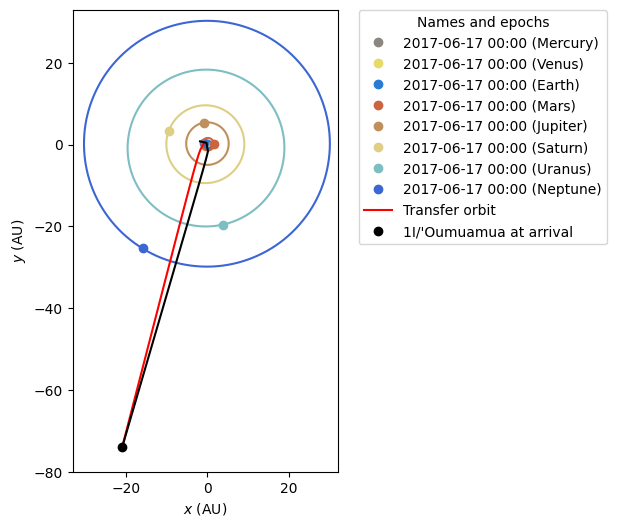
\includegraphics[width=0.9\textwidth]{static/oumuamua/direct-optimum-transfer.png}
  \caption{Optimum direct transfer orbit between Earth and 1I/'Oumuamua. The
    high speed of 'Oumuamua one passing through its perihelion leads to a low
    resolution in the sampling of points close to this region.}
  \label{fig:oumuamua-direct-transfer-orbit}
\end{figure}

Figure \ref{fig:oumuamua-direct-transfer-orbit} shows the trajectory of the
optimum transfer between Earth and 1I/'Oumuamua. Impulses for this maneuver are
described in table \ref{tab:oumuamua-direct-transfer-impulses}. Total cost is
$42.00$ km/s.

\begin{table}[H]
  \centering
  \begin{tabular}{|c|c|c|c|}
    \hline
    Impulse & $\Delta v_x$ [km/s] & $\Delta v_y$ [km/s] & $\Delta v_z$ [km/s] \\
    \hline
    Launch & 28.20 & -30.10 & 3.91 \\
    \hline
    Arrival & 0.28 & -0.49 & -0.02 \\
    \hline
  \end{tabular}
  \caption{Impulses required for the optimum transfer between Earth and 1I/'Oumuamua.}
  \label{tab:oumuamua-direct-transfer-impulses}
\end{table}

This scenario was analyzed by \cite{hein2018} too. However, the analysis
presented in this work expands previous article by covering the retrograde case
and providing the optimum solution.

Despite having found and optimum solution, the value of $C_3 = 720.28$
km$^2$/s$^2$ is still a high value for orbit transfers.

\subsection{Borisov}

Regarding Borisov, the most optimum transfer is also a prograde transfer. The
analysis of figure \ref{fig:borisov-direct-prograde-transfer-porkchop} shows
that the lowest characteristic energy is the one collected in table
\ref{tab:borisov-direct-transfer-optimum}.

Previously found literature shows that \cite{hibberd2021} analyzed the direct
transfer to the interloper, where he states that the optimum transfer happens 

Impulses for this maneuver are described in table
\ref{tab:borisov-direct-transfer-impulses}. Total cost is $36.95$ km/s.

\begin{table}[H]
  \centering
  \begin{tabular}{|c|c|c|c|}
    \hline
    Impulse & $\Delta v_x$ [km/s] & $\Delta v_y$ [km/s] & $\Delta v_z$ [km/s] \\
    \hline
    Launch & -11.92 & 3.69 & -25.73 \\
    \hline
    Arrival & 0.58 & -5.37 & -6.37 \\
    \hline
  \end{tabular}
  \caption{Impulses required for the optimum transfer between Earth and 2I/Borisov.}
  \label{tab:borisov-direct-transfer-impulses}
\end{table}


\vspace{1cm}
\begin{table}[H]
  \centering
  \begin{tabular}{|c|c|c|c|}
    \hline
    Object & Launch date & Arrival date & Required $C_3$ [km$^2$/s$^2$] \\
    \hline
    2I/Borisov & 2016-04-28 & 2032-01-15 & 820.06 \\
    \hline
  \end{tabular}
  \caption{Optimum transfer orbit for a direct transfer between the Earth and 2I/Borisov.}
  \label{tab:borisov-direct-transfer-optimum}
\end{table}

Figure \ref{fig:borisov-direct-transfer-orbit} shows the trajectory of the
optimum transfer between Earth and 2I/Borisov.

\begin{figure}[H]
  \centering
  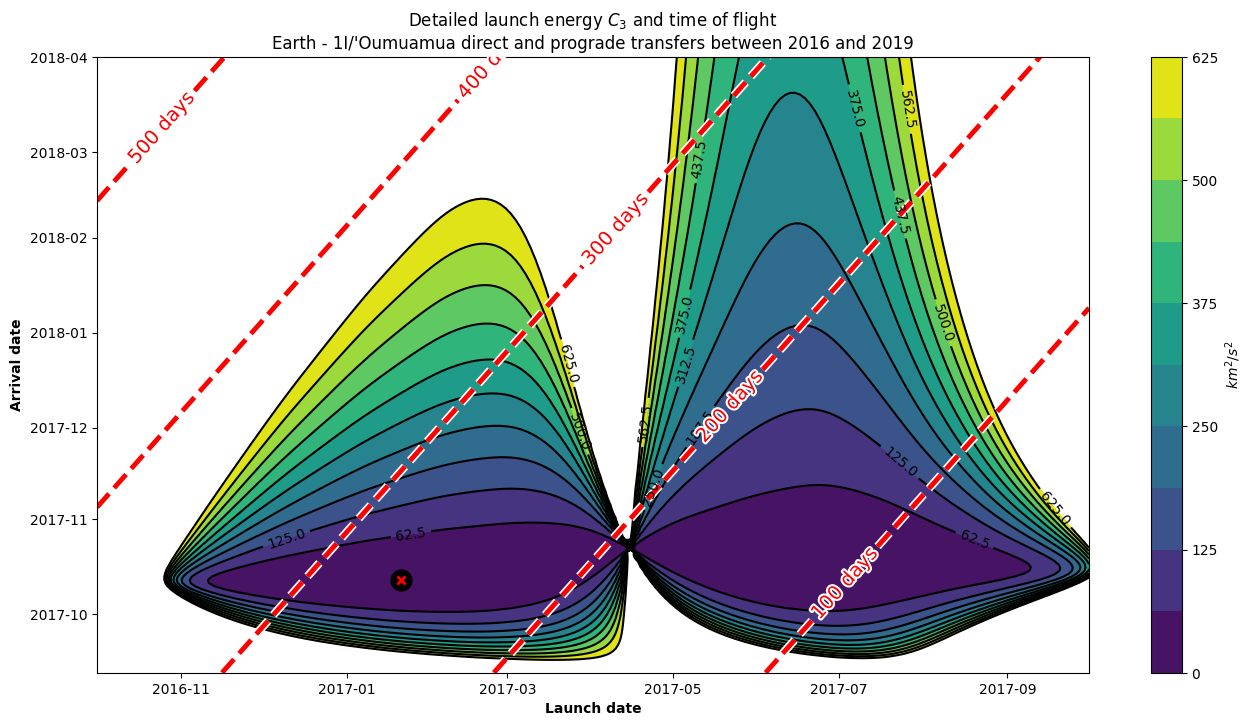
\includegraphics[width=\textwidth]{static/borisov/direct-detailed-porkchop-tof.png}
  \caption{Optimum direct transfer orbit between Earth and 2I/Borisov. This
        trajectory does not pass close to the Sun. However, the transfer requires almost $820$
        km$^2$/s$^2$ to achieve a targeting with the interloper.}
  \label{fig:borisov-direct-transfer-orbit}
\end{figure}

\begin{figure}[H]
  \centering
  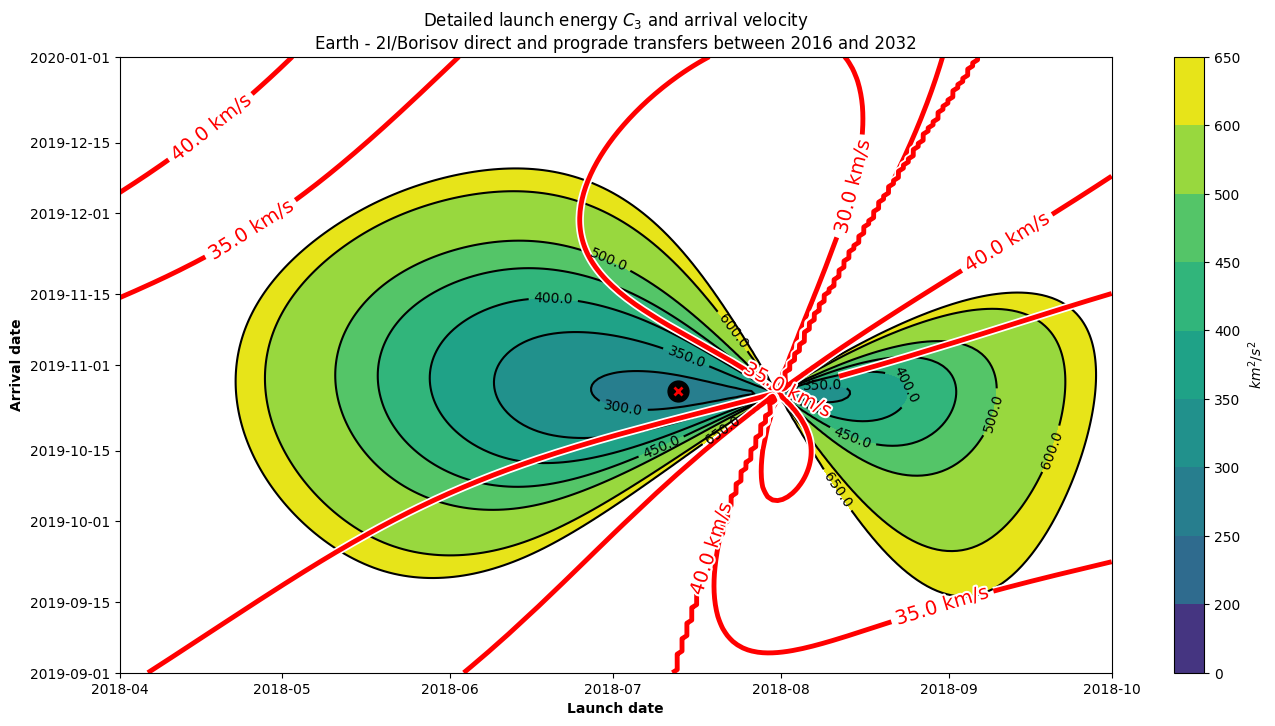
\includegraphics[width=\textwidth]{static/borisov/direct-detailed-porkchop-avl.png}
  \caption{Optimum direct transfer orbit between Earth and 2I/Borisov. This
        trajectory does not pass close to the Sun. However, the transfer requires almost $820$
        km$^2$/s$^2$ to achieve a targeting with the interloper.}
  \label{fig:borisov-direct-transfer-orbit}
\end{figure}

\begin{figure}[H]
  \centering
  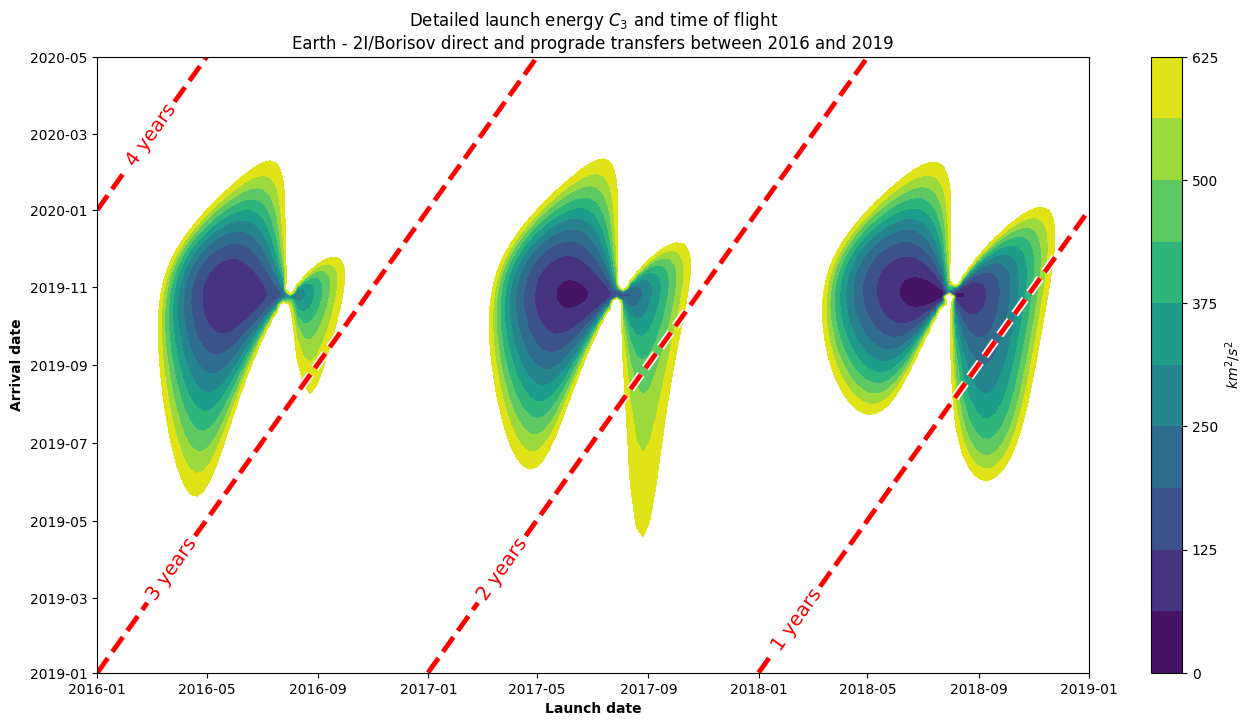
\includegraphics[width=\textwidth]{static/borisov/direct-detailed-porkchop.png}
        \caption[Detailed porkchop showing the optimum transfer for
        2I/Borisov]{The porkchop reveals a series of optimum transfer orbits.
        These values remain suitable for modern chemical propulsion media.}
  \label{fig:borisov-direct-detailed-porkchop}
\end{figure}

